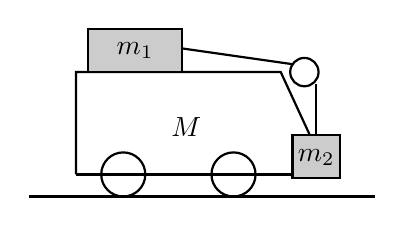
\begin{tikzpicture}[scale=1]
  % cart body
  \draw[thick] (0,0.9) -- (0,2.2) -- (2.6,2.2) -- (3.2,0.9) -- (0,0.9);
  \draw[thick] (0,0.9) -- (3.2,0.9);
  % wheels
  \draw[thick] (0.6,0.9) circle (0.28);
  \draw[thick] (2.0,0.9) circle (0.28);
  % ground
  \draw[thick] (-0.6,0.62) -- (3.8,0.62);
  % block m1 on top of cart
  \draw[thick,fill=gray!40] (0.15,2.2) rectangle (1.35,2.75);
  \node at (0.75,2.47) {$m_1$};
  % pulley at corner
  \draw[thick] (2.9,2.2) circle (0.18);
  % string from m1 over pulley
  \draw[thick] (1.35,2.5) -- (2.75,2.3);
  % hanging string and block m2
  \draw[thick] (3.05,2.05) -- (3.05,1.4);
  \draw[thick,fill=gray!40] (2.75,0.85) rectangle (3.35,1.4);
  \node at (3.05,1.12) {$m_2$};
  % label M for cart
  \node at (1.4,1.5) {$M$};
\end{tikzpicture}
